\chapter{Behold the Glorious Christ (1:1--1:11)}

What does 'glory' mean to us?

In the four Gospels, we encounter Jesus at His first coming to earth. He came among us in humility. He served others, healed the sick, sought the lost, and ultimately ``gave his life as a ransom for many.''

In many Catholic churches, Jesus is depicted upon the cross. A crown of thorns rests upon His head, and His body bears the wounds of the scourging. This is Jesus, the suffering Servant, the One who endured death for our sake. 

It is difficult to reconcile such an image of humility with what we usually think of as glory.

The apostle Paul tells us that Christ was in very nature God, yet He ``made himself nothing by taking the very nature of a servant'' and humbled Himself in obedience, even to death on a cross (Philippians 2:6--8, NIV).

But the story did not end at the cross.

``Therefore God exalted him to the highest place and gave him the name that is above every name, that at the name of Jesus every knee should bow, in heaven and on earth and under the earth.''
---Philippians 2:9--10  

This is the glorious Christ whom Revelation invites us to behold.

From its very opening, Revelation gives us the voice of the risen and glorified Christ. The One who once walked among us in humility now stands before us in majesty, reigning over history and calling His people to see Him as He truly is.

\begin{ScriptureBox}

\item[1:1] The revelation from Jesus Christ, which God gave him to show his servants what must soon take place. He made it known by sending his angel to his servant John,

\item[1:2] who testifies to everything he saw---that is, the word of God and the testimony of Jesus Christ.

\item[1:3] Blessed is the one who reads aloud the words of this prophecy, and blessed are those who hear it and take to heart what is written in it, because the time is near.

\item[1:4] John, To the seven churches in the province of Asia: Grace and peace to you from him who is, and who was, and who is to come, and from the seven spirits before his throne,

\item[1:5] and from Jesus Christ, who is the faithful witness, the firstborn from the dead, and the ruler of the kings of the earth. To him who loves us and has freed us from our sins by his blood,

\item[1:6] and has made us to be a kingdom and priests to serve his God and Father---to him be glory and power for ever and ever! Amen.

\item[1:7] ``Look, he is coming with the clouds,'' and ``every eye will see him, even those who pierced him''; and all peoples on earth ``will mourn because of him.'' So shall it be! Amen.

\item[1:8] ``I am the Alpha and the Omega,'' says the Lord God, ``who is, and who was, and who is to come, the Almighty.''

\item[1:9] I, John, your brother and companion in the suffering and kingdom and patient endurance that are ours in Jesus, was on the island of Patmos because of the word of God and the testimony of Jesus.

\item[1:10] On the Lord's Day I was in the Spirit, and I heard behind me a loud voice like a trumpet,

\item[1:11] which said: ``Write on a scroll what you see and send it to the seven churches: to Ephesus, Smyrna, Pergamum, Thyatira, Sardis, Philadelphia and Laodicea.''

\end{ScriptureBox}

\section{John Recorded Revelation on the Island of Patmos}

John is traditionally associated with five books of the New Testament: the Gospel of John, 1 John, 2 John, 3 John, and Revelation.

During the reign of the Roman emperor, John was exiled to the island of Patmos because of his Christian faith and his testimony to Jesus Christ. It was there that he received and recorded the visions preserved in Revelation.
The circle in Figure~\ref{fig:turkey-seven-churches} marks the island of Patmos,
and the numbers show the seven churches: \ding{172} Ephesus, \ding{173} Smyrna, \ding{174} Pergamum, \ding{175} Thyatira, \ding{176} Sardis, \ding{177} Philadelphia, and \ding{178} Laodicea. 


\begin{figure}[htbp]
    \centering
    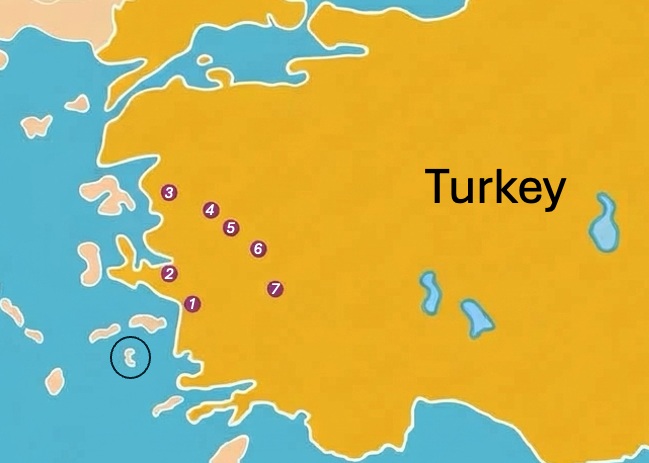
\includegraphics[
        width=0.9\textwidth,
        trim=0 0 0 100,
        clip
    ]{images/turkey}
    \caption{The Seven Churches}
    \label{fig:turkey-seven-churches}
\end{figure}

In such a lonely and troubled place, could the visions John witnessed have been nothing more than hallucinations?

There are good reasons not to dismiss his testimony in this way.

First, John's account does not portray him as someone who had lost consciousness or become detached from what was happening around him. As the visions unfolded, he often knew what he was seeing. He recorded explanations given by angels, asked questions, and received answers. His account presents a witness being shown and instructed, not merely someone recounting a series of bewildering impressions.

Second, Revelation was preserved and transmitted within the early Christian community. In the second century, the church father Irenaeus quoted Revelation repeatedly in his work \textit{Against Heresies}.\footnote{Irenaeus. (1885). \textit{Against Heresies} (A. Roberts \& W. H. Rambaut, Trans.). Christian Literature Publishing. (Original work published ca. 180).} Irenaeus lived relatively close to the apostolic age, and his writings provide important evidence for the early reception of Revelation.

In the fourth century, the church historian Eusebius gathered traditions from the early church in his \textit{Ecclesiastical History}. He recorded traditions concerning John, Patmos, and the period of the emperor Domitian.\footnote{Eusebius. (1890). \textit{Church History} (A. C. McGiffert, Trans.). Christian Literature Company. (Original work published ca. 325).} Eusebius also recorded the tradition that John later returned to Ephesus.\footnote{Eusebius, ca. 325/1885, 3.18.1, 3.20.9.}

Taken together, this early testimony helps establish that Revelation was not a later invention detached from the apostolic church. It was received, preserved, and transmitted as an apostolic witness within the early Christian community.

What, then, is the Christ revealed in this book?

\section{The Glorious Christ}

If the Jesus you know is the suffering Servant, you can be certain that He is also the exalted King.

Colossians 1:15 declares that the Son ``is the image of the invisible God.'' Hebrews 1:3 describes Him as ``the radiance of God's glory and the exact representation of his being''  .

In Revelation 1--3, we encounter one description after another of the glory of Jesus Christ. These descriptions can be brought together in Table~\ref{tab:christ-revelation-1-3}.

\begin{longtable}{p{1.2cm} p{7.8cm}}
\caption{Descriptions of Jesus Christ in Revelation 1--3}
\label{tab:christ-revelation-1-3} \\

\hline
\textbf{Passage} & \textbf{Description of Jesus Christ} \\
\hline
\endfirsthead

\hline
\textbf{Passage} & \textbf{Description of Jesus Christ} \\
\hline
\endhead

\hline
\endfoot

\hline
\endlastfoot

1:5
& The firstborn from the dead. He has conquered death and stands as the beginning of the new creation. \\

3:14
& The ruler of God's creation, supreme over all that has been made. \\

1:8
& The Alpha and the Omega, the beginning and the end. He transcends time and holds history in His sovereign hands. \\

1:13
& One like a son of man, clothed in a robe reaching down to His feet and with a golden sash around His chest. His appearance conveys majesty and evokes the dignity of a royal and priestly figure. \\

1:14
& His head and hair are white like wool, as white as snow. The imagery conveys holiness and majesty and recalls the Ancient of Days in Daniel's vision. \\

1:14; 2:18
& His eyes are like blazing fire. Nothing is hidden from His sight. He searches the human heart and sees the truth about every person and every church. \\

1:15; 2:18
& His feet are like bronze glowing in a furnace. The imagery suggests strength, purity, and the authority to execute righteous judgment. \\

1:15
& His voice is like the sound of rushing waters, conveying overwhelming majesty and authority. \\

1:16; 2:1; 3:1
& He holds the seven stars in His right hand and walks among the seven golden lampstands. He holds the seven stars and the seven spirits of God. These images portray His authority over the churches, His presence among them, and His sovereign rule. \\

1:16; 2:12
& A sharp double-edged sword comes from His mouth. His word exposes error, judges evil, and defeats His enemies. \\

1:16
& His face shines like the sun in all its brilliance, revealing His divine majesty and glory. \\

1:18
& He holds the keys of death and Hades, demonstrating His authority over death and the realm of the dead. \\

3:7
& He holds the key of David. As the rightful King, He opens what no one can shut and shuts what no one can open. \\

3:14
& He is the faithful and true witness, wholly trustworthy in all He reveals and declares. \\

\end{longtable}

\section{The Old Testament Foretold the Glory of Christ}

The glorious Christ John describes bears a striking resemblance to the figures and visions seen by Old Testament prophets centuries earlier.

This is no coincidence. Jewish readers familiar with the Scriptures would recognize in Revelation's portrayal of Christ the glorious King whom the Old Testament had anticipated and promised.

\begin{itemize}
    \item \textbf{Daniel 7:9.} ``As I looked, thrones were set in place, and the Ancient of Days took his seat. His clothing was as white as snow; the hair of his head was white like wool. His throne was flaming with fire, and its wheels were all ablaze.''  

    \item \textbf{Daniel 7:13.} ``In my vision at night I looked, and there before me was one like a son of man, coming with the clouds of heaven.''  

    \item \textbf{Daniel 7:14.} ``He was given authority, glory and sovereign power; all nations and peoples of every language worshiped him. His dominion is an everlasting dominion that will not pass away, and his kingdom is one that will never be destroyed.''  

    \item \textbf{Daniel 10:6.} ``His body was like topaz, his face like lightning, his eyes like flaming torches, his arms and legs like the gleam of burnished bronze, and his voice like the sound of a multitude.''  

    \item \textbf{Ezekiel 43:2.} ``And I saw the glory of the God of Israel coming from the east. His voice was like the roar of rushing waters, and the land was radiant with his glory.''  

    \item \textbf{Isaiah 22:22.} ``I will place on his shoulder the key to the house of David; what he opens no one can shut, and what he shuts no one can open.''  
\end{itemize}

These prophets received visions of divine glory in troubled times. The Lord of glory had not forgotten His servants. Rather, He revealed His majesty to them, becoming their strength and their hope.

If the Jesus in your imagination is only the suffering figure who was rejected, abandoned, and nailed to the cross, you need to remind yourself of the greater truth: He is the image of God, the risen and victorious Lord who reigns in glory.

When we come to know Christ in His glory, we discover a hope that sustains us through present suffering, a strength that upholds us in weakness, and a faithfulness that endures even in darkness. We can remain steadfast because the One who walks among His churches is the One who conquered death and will come again.

\section*{Discussion Questions}

\begin{enumerate}
    \item The same Christ who took the form of a servant, suffered for us, was rejected, and died on the cross now reigns in glory and rules over the kings of the earth. How do these two sides of Jesus help us know Him better?
    
    \item Jesus is the First and the Last, He rose from the dead, and He holds the keys of death and Hades. How does this help us stay faithful in hard times?

    \item If we know that one day we will reign with Christ and serve in the presence of God, how should that hope shape the way we live today as people who belong to Him?
\end{enumerate}